\documentclass{article}
\usepackage[utf8]{inputenc}
\title{Video 1: non-pamaetric testing the permutation test. }
\author{wbg231 }
\date{December 2022}
\newcommand{\R}{$\mathbb{R}$}
\newcommand{\B}{$\beta$}
\newcommand{\A}{$\alpha$}
\newcommand{\D}{\Delta}

\newcommand{\avector}[2]{(#1_2,\ldots,#1_{#2})}
\newcommand{\makedef}[2]{$\textbf{#1}$:#2 }
\usepackage{tikz,graphicx,hyperref,amsmath,amsfonts,amscd,amssymb,bm,cite,epsfig,epsf,url}

\begin{document}

\maketitle

\section{introduction}
\begin{itemize}
\item \href{https://www.youtube.com/watch?v=frSkAi36qd0}{vedio link}
\subsection{hyptoshsi testing }
\item steps of hypothsis testing framework 
\begin{enumerate}
    \item chose a conjectture ie allternative hypothsis $H_{1}$
    \item chose a null ie $H_{0}$
    \item chose a test stat (should be large if there is a lot of evedince against the null) 
    \item decide on a signefgence level
    \item gater data and compute test stat 
    \item compute the p value 
    \item reject the null if $\text{p-value}\leq \alpha$

\end{enumerate}
\subsection{p-value}
\item the p-value is the probability of observing a larger or equal test stat under the null hypothesis
\item the issue with that is we need to know how the test stat is distributed under the null 
\item what if we do not know this?
\subsection{price of burgers example}
\item suppose we have a conjecture that burgers in NYC are more expensive  than those in madrid 
\item null is that the price of burgers in both cities has the same distribution 
\item the test stat is average price of burger in nyc - average price of burger in madrid 
\item this would be high if the alternative holds and low otherwise
\item suppose we see two places in nyc that charge 16 and 18 dollars each 
\item and two places in madrid charge 13 dollars each 
\item $d_{data}=m(ny)-m(\text{Madrid})=4$
\item is this evedince against the null? we dont know with out a p-value 
\item but we do not know how our test stat is distributed under the null
\subsection{key idea}
\item if the price distribution is the same in both cities where the burgers came from should not matter
\item that is we should be able to switch around the labels and if it holds we would have been 
equally likely to observe that data as well
\item so we can look at all permutations of the labels and there corresponding test statistics
\item here are all possible realizations of the test stat 
\item 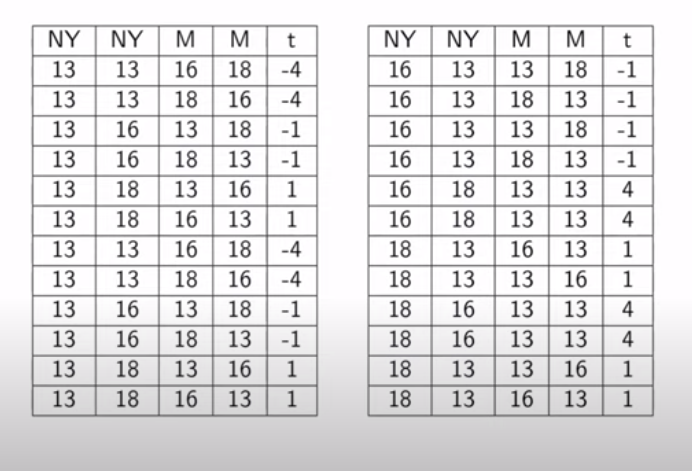
\includegraphics[width=10cm]{notes/week_7/vedio_1/immages/vedio-1-1.png}
\item so now we want to know how unlikely was the data we saw. 
\item that is how many of these permutations have a test stat larger or equal to that we actual observed in the data (4)? it was like 16.7\%
\item this is not quite the same 
\subsection{multiset of permutations}
\item for any $x\in \mathbb{R}^{d}\Pi_{x}$ is a multiset of $d!$ perumations
\item 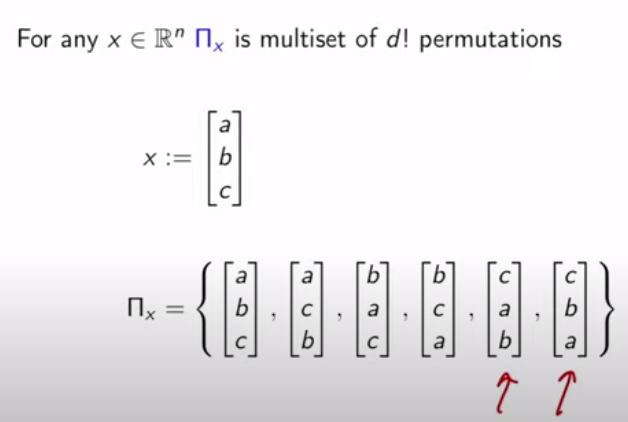
\includegraphics[width=10cm]{notes/week_7/vedio_1/immages/vedio-1-2.png}
\item so noice here that the last two ellements of the multiset are the same, so it is not a propper set 
\subsection{p-value of permuation test}
\item if our observed data is $x_{data}\in \mathbb{R}^{d}$
\item and we have observed test stat $t_{data}:=T(x_{data})$
\item and we mode the distribution of the data under the null ypothsis as a random vector $\Tilde{x}_{null}$
\item then our test stat unde rthe null we call $\Tilde{t}_{null}=T(\Tilde{x}_{null})$
\item so our p value function in this case is $pv(t):=P(\Tilde{t}_{null}\geq t |\Tilde{x}_{null}\in \Pi_{x_{data}})$
\item so that is the p -value is teh probaility that t under the null is greater than that value given teh data we observed is a a permuation of the observed data
\item in the typical p-value we do not condtion on this, but this is required for the permuation test 
\subsection{exchangability}
\item the enteries of $\Tilde{x}$ are exchangable if permuting them does not change the distrobution of $\Tilde{x}$
\item $\Pi_{x}$ the multset of permautions of x 
\item the enteries fo a discrete random vector $\Tilde{X}$ are exchangable if $$\forall v\in \Pi_{x}, P_{\Tilde{x}}(x)=P_{\Tilde{x}}(v)$$
\item so that means changing the order  of ellements does not change the distrobution of the vector
\item the same holds for continous rv
\subsection{idd rvs}
\item exhangability will hold for iid rvs 
\item we the entries are indepdent then the joint is the product of the marginals then if they are identically distributed it is the asme as the marginal of eahc multiples toghter. then if we look at any vecotr in the multset so exchangability holds
\item if $\Tilde{x}_1...\Tilde{x}_{d}$ are iid 
\item then $f_{\tilde{x}}(X)=\ \Pi_{i=1}^{d}f_{\Tilde{x}_i}(x_i)=\Pi_{i=1}^{d}f_{marg}(x_i)=\Pi_{i=1}^{d}f_{marg}(v_i)=f_{\Tilde{x}}(x), \forall v \in \Pi_{x}$
\subsection{consequnces of exhangability}
\item if $\Tilde{x}_{null}$ is exhangeable then the p values are unfiorm that is 
\item $P(\Tilde{x}_{null}=v|\Tilde{x}_{null}\in \Pi_{x_{data}})=\frac{1}{n!}, \forall v \in \Pi_{x} $
\item this holds pretty directly from the defention of exhangability
\item furhter then we know the sum of the condtionals of each value in the multiset  add up to 1 
\item once again this holds pretty directly from the defention
\item the real point is that the liklhood of seing any perumation is equal 

\subsection{nonparametric p value function}
\item this is important because it allows us to comptue the distribution of our p values even when we do not have acess to the distribution of the test stat under the null 
\item bascailly our p value of an event is the number of times that events occours over the total number of events (N!)
\item more specfically we can write out our p value function as  $pv(t)=P(T(\Tilde{x}_{null})\geq t|\Tilde{x}_{null} \in \Pi_{x_{data}})=P(\cup_{v\in \Pi_{x_{data}}:T(v)\geq t}|\Tilde{x}_{null} \in \Pi_{x_{data}})=
\Sigma_{v\in \Pi_{x_{data}}:T(v)\geq t}P(\Tilde{x}_{null}=v|\Tilde{x}_{null} \in \Pi_{x_{data}})=\frac{\Sigma_{v\in \Pi_{x_{data}}} \mathbb{I}(T(v)\geq t)}{n!}$
\item we are more or less saying if the enteries are exchangable under the null than we would be equally likely to see any outcome, and to comptute the condtional prob the test stat is greater than what we saw than we kust need teh number of cases where the test stat is greater than or equal to what we saw over the liklyhood of seing it whcih is 1 over the number of permutations
\subsection{false postive} 
\item the point of all of this is that this re-defined p -value still allows us to garuntee that $P(\text{false postive}\leq \alpha)$
\item this holds from a really close argument to what works with the regular p -value
\item our new defention of p-value using this condtional arugment still lets us maintain the liklyhood of a false postive being upper boudned by the signefgence level
\subsection{free throws examples}
\item we are doing the free throw example that we have done in the past few vedios
\item so assume we have the same set up
\item unde the null the free throws are iid 
\item in our data he shoots 44 free throws at home and 41 away
\item so under the permuation test we can write our data as $\Tilde{x}_{data}=\begin{pmatrix}
   1\\0\\0\\...\\1 
\end{pmatrix}$ which is of length (85) ie the number of shots at home pluess the number of shots away and where the liklhood of any permuation is equally
\item so our test stat can be expressed as $T(v)=\frac{1}{44}\Sigma_{i=1}^{44}v[i]-\frac{1}{41}\Sigma_{i=45}^{85}v[i]$ where i is any random permuation of our input vector 
\item then our p value is $pv(t)=\frac{\Sigma_{v\in \Pi_{x_{data}}}\mathbb{I}(T(v)\geq t)}{n!}$

\item the issue with this is that there are 85 data points and $85!$ is way to high to compute 
\item so we an use montecarlo simulation to take some random subset of the multiset to aproimate this (that is the jack knife)
\subsection{parametric two sample vs nonparametric permuation test for free throws example}
\item 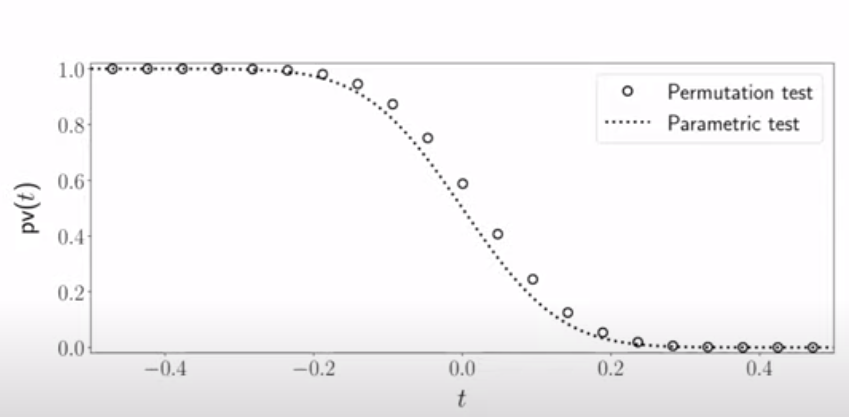
\includegraphics[width=10cm]{notes/week_7/vedio_1/immages/vedio-1-3.png}
\item here we have plotted the p-value function for both tests 
\item they are super similar 
\item but the permuation test is a lot more simple 
\item this is a numerical aproximation that aproximates an analytical solution very well 
\item the nice thing about this test is that it is easy and works pretty well in a lot of cases 
\item after this he doss an example with the median i think it is worth watching if you are intrested i am not going to write it down tho. 



\end{itemize}

\end{document}
